%------------------------------%
%% ✎ Dylan (V1) %%%%%%%%% ✅ %%
%% ✎ Alain (V2) %%%%%%%%% ❌ %%
%% ✎ Dylan (V3) %%%%%%%%% ❌ %%
%------------------------------%

\afterpage{%
%\afterpage{%

    % Arrière-plan partie I
    \AddToShipoutPictureBG*{%
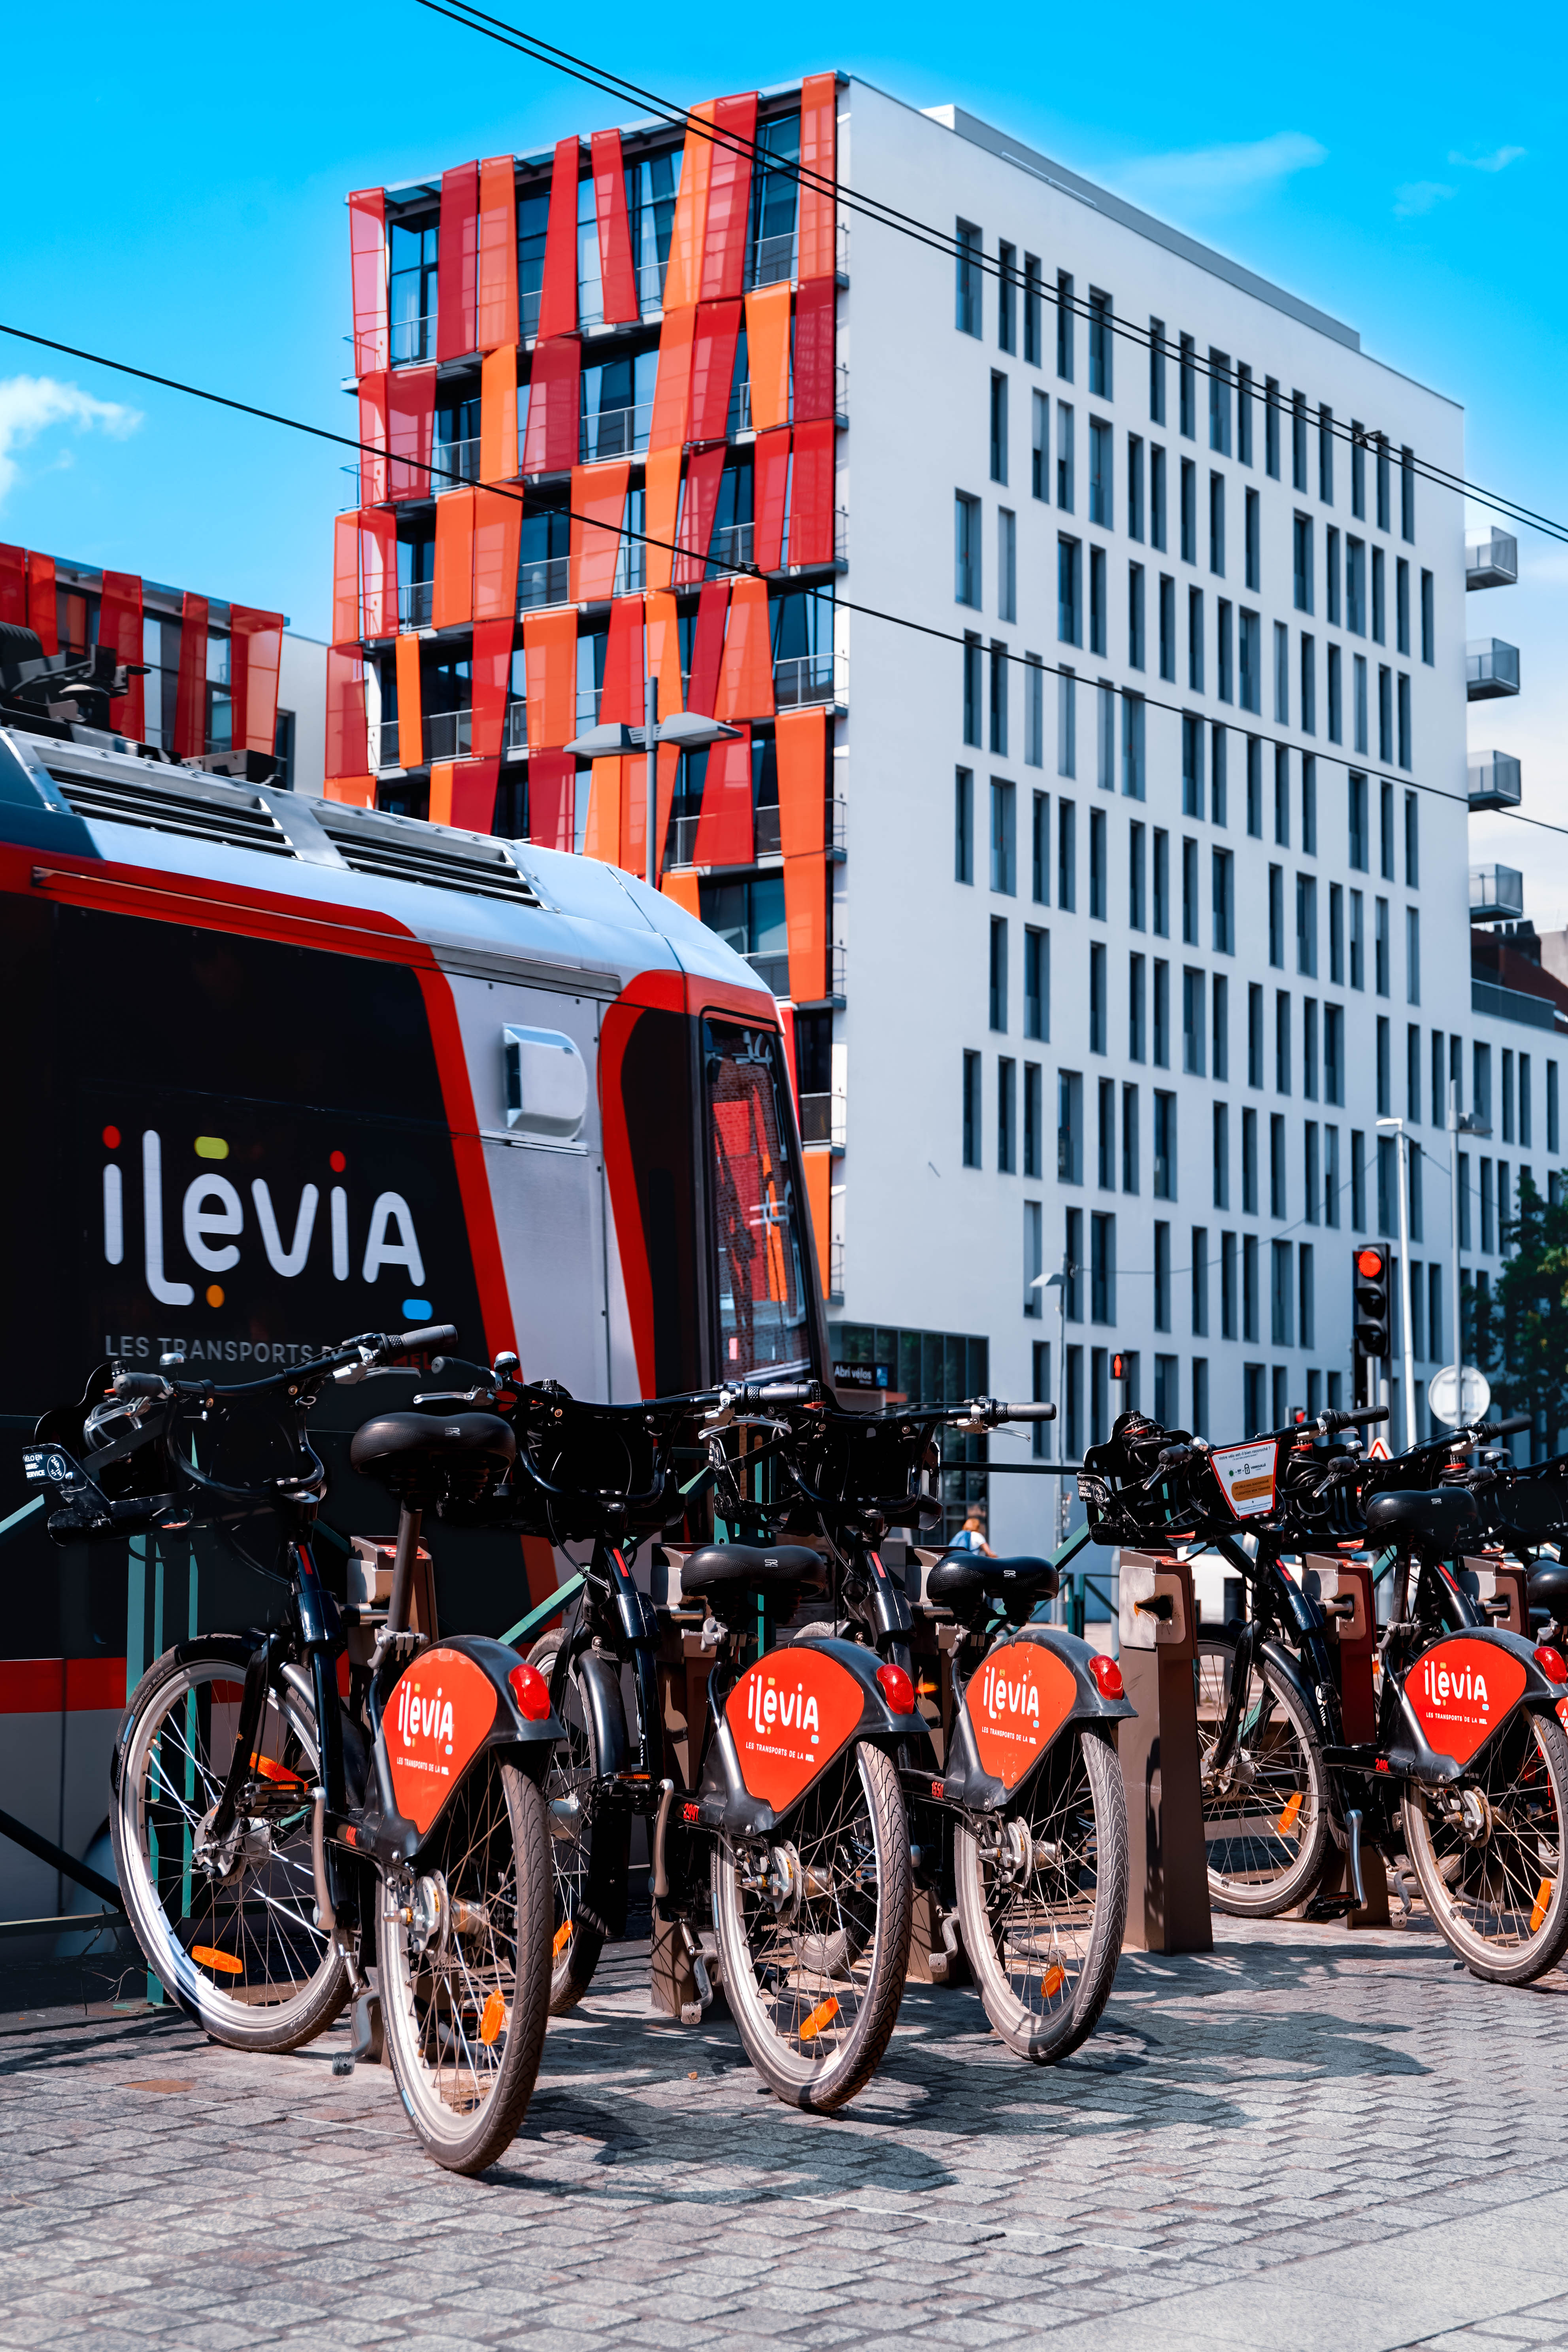
\includegraphics[width=\paperwidth,height=\paperheight]{src/Figures/Arriere_plan/Arriere_plan_Part_1.jpg}
    }

% Rectangle
\AddToShipoutPictureBG*{
  \begin{tikzpicture}[remember picture,overlay]
    \node[fill=white, opacity=0.75, text width=\paperwidth, minimum height=10cm, anchor=north] 
    at ([yshift=-7.7cm]current page.north) {};
  \end{tikzpicture}
}

% Source
\AddToShipoutPictureFG*{
  \AtPageLowerRight{
    \raisebox{1cm}{
      \hspace{16cm}
      
\begin{tikzpicture}
        \node[fill=white, rounded corners=5pt, inner sep=5pt, align=center] {
          \tiny{Photographie~: \textcolor{blue}{Dylan Moinse (2021)}}
        };
      \end{tikzpicture}
    }
  }
}
}%}

\renewcommand{\thefigure}{\thechapter.\arabic{figure}} % Numérotation standard
\renewcommand{\thetable}{\thechapter.\arabic{figure}}
\setcounter{figure}{0}

\needspace{1\baselineskip} % Réserve de l'espace
\part{Cadres théorique et méthodologique pour une intégration de la mobilité individuelle légère en vue d'un urbanisme orienté vers le rail
    \label{part1:titre}
    }
    \markboth{Partie~I~: Cadres théorique et méthodologique de la recherche}{}
    \markright{Partie~I~: Cadres théorique et méthodologique de la recherche}{}

% Introduction de la partie I
\cleardoublepage
\section*{Introduction de la partie~I
    \label{part1:introduction}
    }
    \addcontentsline{toc}{chapter}{Introduction de la partie~I}

    % Introduction
\lettrine[lines=3, findent=8pt, nindent=0pt]{\lettrinefont L}{intégration} de la mobilité individuelle légère dans les quartiers de gare et son rôle dans une relecture du \acrfull{TOD} s’inscrivent dans une réflexion plus large sur les interactions entre urbanisme, configurations territoriales, infrastructures de transport et pratiques de mobilité. Avant d’engager la construction d'un matériau empirique et son analyse, il est essentiel de revenir sur les fondements théoriques, les évolutions conceptuelles et les méthodes d’investigation qui structureront cette recherche. Cette première partie vise ainsi à établir un cadre théorique et méthodologique, permettant de comprendre les enjeux de l’accessibilité intermodale et d’explorer les modalités d’intégration de la mobilité individuelle légère dans les stratégies d’aménagement et de transport. Elle repose sur une articulation entre trois dimensions~: (i) une revue conceptuelle des modèles urbains et de leur adaptation aux dynamiques contemporaines de mobilité~; (ii) un état de l’art des recherches existantes sur l’intermodalité et la complémentarité entre mobilité individuelle et transport public~; (iii) une structuration méthodologique détaillant les approches, les outils et les techniques d'analyse mobilisés pour appréhender ces transformations. En rassemblant ces éléments, cette première partie ancre la réflexion dans un cadre structuré, justifiant l'intérêt de nous intéresser au \acrshort{TOD} non pas comme un modèle urbain figé, mais comme une stratégie évolutive, capable d’intégrer la mobilité individuelle légère pour en maximiser les bénéfices attendus.%%Rédigé%%

    % Chapitre 1
\textsl{Éclairer l'évolution conceptuelle de l'urbanisme ferroviaire au regard de ses réajustements} (\hyperref[objectif-1]{objectif~\(O_1\)}, page~\pageref{objectif-1}). \hyperref[chap1:titre]{Le premier chapitre} (page~\pageref{chap1:titre}) retrace l’évolution du \acrshort{TOD} en tant que modèle d’aménagement structurant le développement urbain régional autour du réseau de transport en commun. Il en analyse les principes fondamentaux, parmi lesquels figurent la densification autour des pôles de transport, la mixité fonctionnelle et le traitement des espaces publics comme leviers de territoires moins dépendants de l'automobile. Malgré ses ambitions, le \acrshort{TOD} présente plusieurs limites structurelles, notamment en matière d’accessibilité. Si son efficacité est avérée dans des contextes métropolitains denses, où les infrastructures de transport public sont bien connectées au tissu urbain, elle s’avère moins évidente dans les territoires périurbains, où la dépendance à l’automobile reste prégnante. La principale cause réside dans la mise à l'écart de solutions intermodales adaptées aux \Guillemets{premiers et derniers kilomètres}. Cette situation limite ainsi les effets positifs escomptés du \acrshort{TOD} en matière de report modal et d’optimisation des réseaux de transport. C’est dans ce contexte que la mobilité individuelle légère~–~ englobant le vélo, la trottinette et d'autres dispositifs de micro-mobilité qui impliqueront à leur tour une remise en perspective de leur évolution~–~apparaît comme un levier stratégique pour compléter et réactualiser le \acrshort{TOD}. Son intégration aux politiques d’aménagement et de transport pourrait permettre de combler les lacunes du modèle traditionnel, en assurant un système de mobilité alternatif plus efficace et en phase avec les aspirations qui ont émergé. Toutefois, cette complémentarité reste encore peu explorée dans les travaux académiques et insuffisamment mise en œuvre dans les politiques publiques. Une fois démontré l’intérêt du \acrshort{TOD} comme cadre théorique pour répondre aux impératifs de réduction de l’usage automobile, il convient d’en interroger l’adaptabilité dans des territoires historiquement conçus pour l’automobile. Cette réflexion conduit ainsi à examiner les travaux existants sur cette problématique et à tirer les enseignements nécessaires afin d’orienter notre propre investigation.%%Rédigé%%

    % Chapitre 2
\textsl{Synthétiser les pratiques de recherche et les connaissances actuelles sur un urbanisme orienté vers les transports en commun et prenant appui sur la mobilité individuelle légère} (\hyperref[objectif-2]{objectif~\(O_2\)}, page~\pageref{objectif-2}). \hyperref[chap2:titre]{Le deuxième chapitre} (page~\pageref{chap2:titre}) constitue une \acrfull{RSL} conçue pour mieux comprendre les synergies possibles entre le \acrshort{TOD} et la mobilité individuelle légère. Nous employons dans ce cadre une démarche scientométrique dans le but d’identifier les grandes tendances de la recherche à propos de ce sujet de recherche et d’analyser l’évolution des objets qui y sont associés. Ce chapitre vise à recenser et à cartographier les travaux mobilisant, implicitement ou explicitement, les contours d’un \acrshort{B-TOD} ou d’un \acrshort{M-TOD}. Il porte son attention non seulement sur les dynamiques géographiques et temporelles des publications et sur leur sémantique, mais également sur les méthodes employées dans ces recherches, afin d’en saisir les approches analytiques et les cadres méthodologiques sous-jacents. L’analyse de ces évolutions permet d’affiner la compréhension des pratiques de mobilité intermodale, en intégrant une lecture plus fine des usages et des déterminants spatiaux de l’accessibilité intermodale. Enfin, cette revue critique de la littérature met en évidence les défis encore non résolus, tant sur le plan conceptuel que dans sa mise en application. Elle soulève plusieurs questions structurantes pour les analyses à venir, en identifiant des lacunes scientifiques et méthodologiques qui guideront le travail empirique de cette recherche. Cet état de l’art constitue ainsi un préalable à l'enquête empirique, en s’appuyant sur les manques identifiés dans la littérature pour proposer une approche renouvelée, à même de mieux saisir les enjeux d'un \acrshort{M-TOD}.%%Rédigé%%

    % Chapitre 3
\textsl{Développer une méthodologie intégrant des approches complémentaires pour aboutir à une étude plus approfondie et en extraire des résultats supplémentaires} (\hyperref[objectif-3]{objectif~\(O_3\)}, page~\pageref{objectif-3}). \hyperref[chap3:titre]{Le troisième chapitre} (page~\pageref{chap3:titre}) sert à répondre empiriquement aux questionnements soulevés dans les chapitres précédents. Pour cela, nous avons conçu et adapté un dispositif méthodologique original. Ce chapitre expose ainsi le cadre méthodologique adopté dans cette thèse. Il s’agit tout d’abord de définir et de justifier le choix du terrain d’étude, tant du point de vue des objets analysés que de celui du terrain géographique concerné. La construction de notre matériau empirique se traduit par la mobilisation d'approches mixtes, mettant en dialogue l'exploitation de bases de données, d'une enquête à la fois quantitative et qualitative ainsi que d'une modélisation spatiale. La méthodologie ainsi décrite permet ainsi d'articuler trois niveaux d'analyse complémentaires~: un niveau comportemental, portant sur les choix modaux et les stratégies de mobilité~; un niveau infrastructurel, explorant les conditions d'accessibilité physiques et organisationnelles~; et un niveau territorial, évaluant l'impact potentiel et effectif et de la mobilité individuelle légère sur les quartiers de gare. Par ailleurs, ce chapitre explicite les moyens mis en œuvre pour traiter les données récoltées, à savoir les outils et les techniques d'analyse mobilisés, à l'interface entre les sciences géographique, sociologique, économique et les sciences de la donnée.%%Rédigé%%